

\section{Environments}\label{apx:scenarios}

\begin{table}[htbp]
  \centering
  \caption{Comparison of Multi-Agent Reinforcement Learning Environments/Frameworks}
  \label{tab:marl_comparison}
  % Optional: resizebox to fit width if needed
  \resizebox{\textwidth}{!}{% 
  \begin{tabular}{@{}l l l l l l l l@{}}
    \toprule % Use booktabs rule, or \hline\hline
    \textbf{Feature} & \textbf{VMAS} & \textbf{PettingZoo} & \textbf{SMAC} & \textbf{MA-MuJoCo} & \textbf{PyBullet} & \textbf{Neural MMO} & \textbf{Melting Pot} \\
    \midrule % Use booktabs rule, or \hline
    Key Focus & Fast, Vectorized & Standardized & StarCraft II & Multi-Agent & General 3D & Large-Scale Agent & Social Dilemmas \\
     & 2D Physics & MARL API & Micromanagement & Robotics (MuJoCo & Physics & Survival/Econ. & / Cooperation \\
     & (PyTorch) & (Collection) & & tasks) & Engine & & \\
    \midrule % Separator line
    Single/Multi & Primarily Multi & Primarily Multi & Multi Only & Primarily Multi & Both & Multi Only & Multi Only \\
     & (can do Single) & (API standard) & & (adaptations) & & (Massively) & \\
    \midrule % Separator line
    Differentiable & Yes & No & No & No & No (standard & No & No \\
     & & & & & use) & & \\
    \midrule % Separator line
    Generality & Medium & Very High (via & Low (Specific game & Medium (MuJoCo & High & Medium (Large- & Medium (Social \\
     & (Physics-based, & wrapped envs) & benchmark) & robotics) & (General & scale agent focus) & dilemmas focus) \\
     & PyTorch) & & & & physics) & & \\
    \bottomrule % Use booktabs rule, or \hline
  \end{tabular}
  } % Closing bracket for resizebox, if used
\end{table}

\begin{figure}[t]
    \centering
    \begin{subfigure}{0.24\textwidth}
        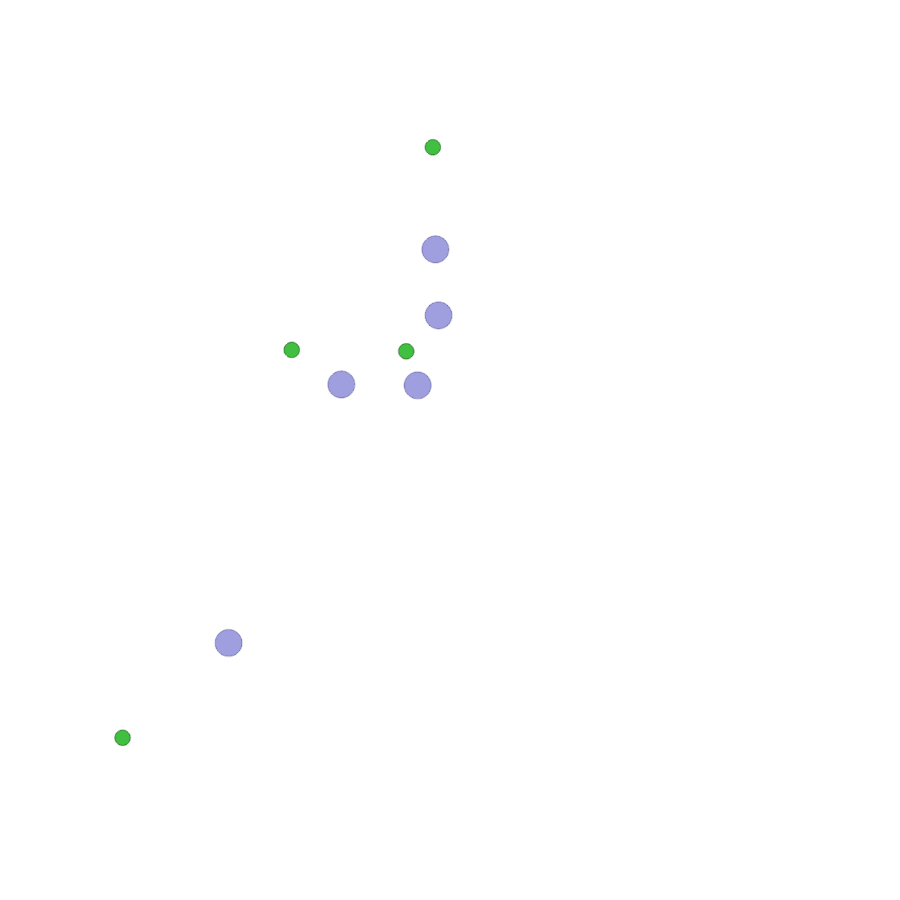
\includegraphics[width=\textwidth]{figs/dispersion.png}
        \caption{Dispersion}
        \label{fig:dispersion}
    \end{subfigure}
    \begin{subfigure}{0.24\textwidth}
        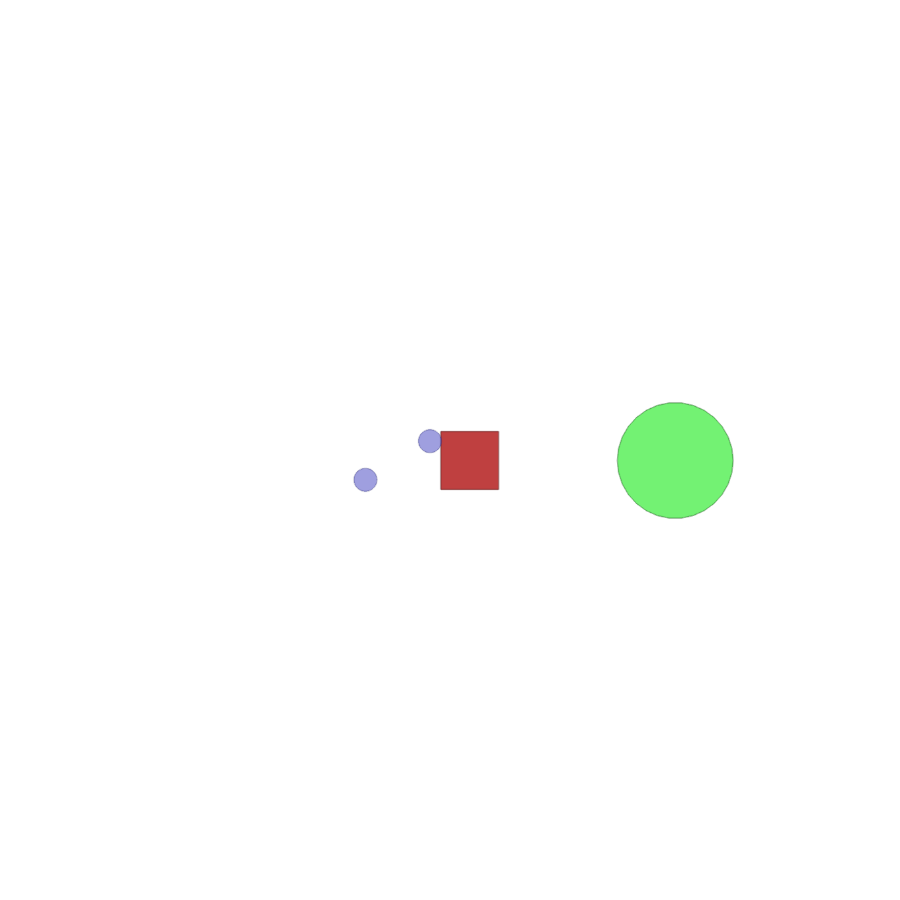
\includegraphics[width=\textwidth]{figs/transport.png}
        \caption{Transport}
        \label{fig:transport}
    \end{subfigure}
    \begin{subfigure}{0.24\textwidth}
        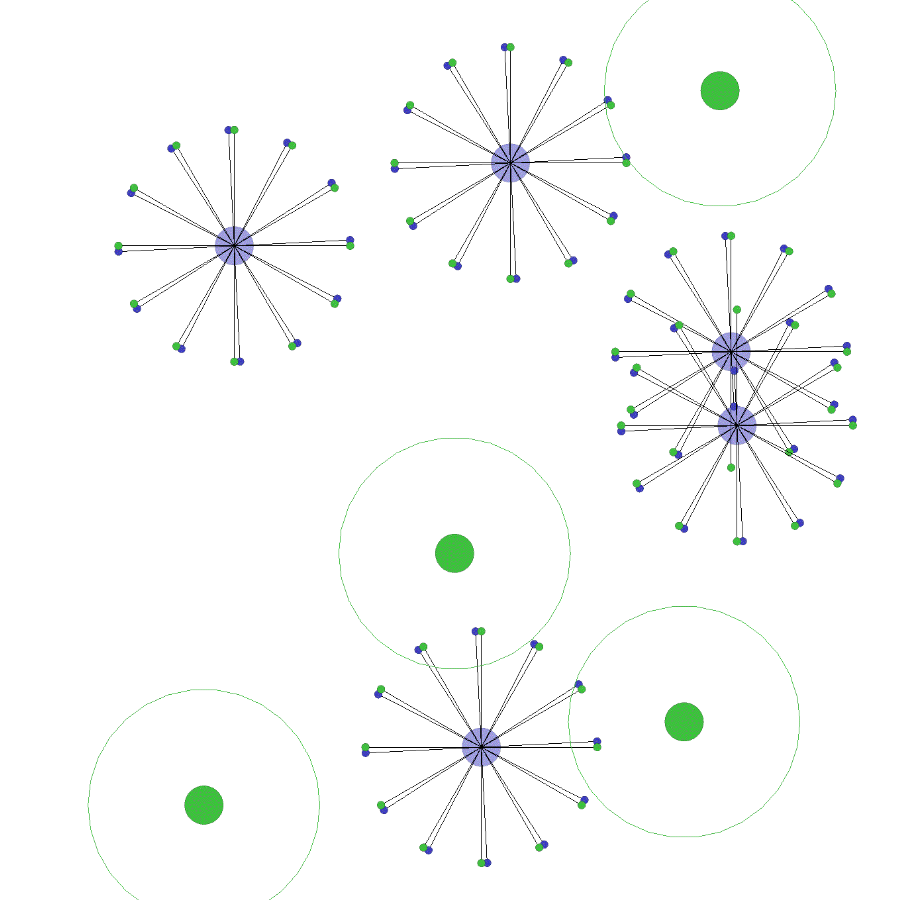
\includegraphics[width=\textwidth]{figs/discovery.png}
        \caption{Discovery}
        \label{fig:discovery}
    \end{subfigure}
    \begin{subfigure}{0.24\textwidth}
        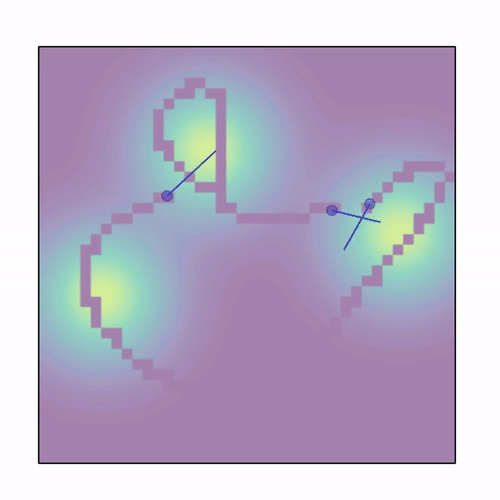
\includegraphics[width=\textwidth]{figs/sampling.png}
        \caption{Sampling}
        \label{fig:sampling}
    \end{subfigure}
    \caption{VMAS environments used in the experiments.}\label{fig:scenarios}\vspace{0.5cm}
\end{figure}

In this section, we provide a detailed overview of the environments used to evaluate the \fname{} algorithm. For our experiments, we selected four vectorized scenarios from VMAS (Vectorized Multi-Agent Simulator), which offers an ideal balance of features for our research objectives.

VMAS stands out among alternative multi-agent reinforcement learning frameworks such as PettingZoo~\cite{DBLP:conf/icml/PettingZoo}, SMAC~\cite{DBLP:conf/icml/ZhangZLZ20}, MA-MuJoCo~\cite{DBLP:conf/aaai/GuptaK0G20}, PyBullet~\cite{DBLP:journals/corr/abs-1710-06347}, Neural MMO~\cite{DBLP:conf/aaai/DiehlB21}, and Melting Pot~\cite{DBLP:conf/icml/GuptaK0G20}. As summarized in Table~\ref{tab:marl_comparison}, VMAS provides several key advantages for our work:

\begin{compactitem}
    \item \textbf{Multi-Agent Framework}: VMAS is specifically designed for multi-agent scenarios, making it appropriate for our experimental setup.
    \item \textbf{Differentiable Physics}: Unlike most alternatives, VMAS offers a differentiable physics engine that enables gradient-based optimization techniques.
    \item \textbf{Vectorized Implementation}: The framework supports parallel execution of multiple environments, significantly improving training efficiency.
    \item \textbf{Physics-based Simulation}: VMAS provides realistic modeling of agent interactions and dynamics through its physics engine.
    \item \textbf{Open Source Accessibility}: The codebase is fully accessible, allowing necessary modifications for our experiments.
\end{compactitem}

While VMAS provides differentiable transition functions across all tasks, its reward functions are generally non-differentiable. To address this limitation, we implemented custom differentiable reward functions where possible to replicate the original VMAS behavior. Consequently, some scenarios are compatible with all tested algorithms (PPO, SHAC, and \fname{}), while others can only be used with PPO and \fname{}.

An additional consideration is that VMAS often provides agents with partial observations rather than complete state information. In some scenarios, these observations contain sufficient information to predict subsequent states, while in others they do not. This partial observability presents a particular challenge for \fname{}, as its world model must operate with incomplete information. In contrast, SHAC computes gradients with access to the full world state. We deliberately maintained these observability constraints to assess \fname{}'s performance under more realistic conditions.

Figure~\ref{fig:scenarios} illustrates the four VMAS environments used in our experiments, which are detailed in the following subsections.

\subsection{Dispersion}
In the Dispersion task, $n$ agents must reach $n$ randomly placed goals. In \Cref{fig:dispersion}, the agents are represented by blue dots, while the goals are depicted as green dots.

Each agent has a continuous 2-dimensional action space, bounded between $-1$ and $1$, to represent acceleration along the x- and y-axes, respectively. Each agent observes its own position, velocity, and relative position to each goal. As a consequence, the world model has sufficient information to accurately predict the next states.

Each agent receives a reward of $1$ upon reaching a goal, making the maximum possible reward $n$. While the transition function is differentiable, the reward function is not. Consequently, only PPO and \fname{} are applicable to this scenario.

\subsection{Transport}
In the Transport problem, $n$ agents work together to push a package to a randomly placed target location. In \Cref{fig:transport}, the agents are represented by blue dots, the package is shown as a red square, and the goal is depicted as a green circle. The more agents collaborate to push the package, the faster they can reach the goal and achieve the maximum reward.

Each agent has a continuous 2-dimensional action space, bounded between $-1$ and $1$, to represent acceleration along the x- and y-axes, respectively. Each agent observes its own position, velocity, the relative position to the package, and the relative position between the package and the goal. As a consequence, the world model has sufficient information to accurately predict the next states.

Each agent receives a reward proportional to the distance between the initial position of the package and the goal. Consequently, the maximum reward corresponds to the distance between the package and the goal. Since the maximum reward varies across environments, we only plot a reference line representing good performance. Although this reward function is differentiable, the implementation provided by VMAS is not. Therefore, we created a custom reward function to replicate the original one used by all algorithms (\fname{}, SHAC, and PPO).


\subsection{Discovery}
In the Discovery task, $n$ agents aim to collect as many randomly placed goals as possible. When they successfully collect $k$ goals, another $k$ goals are randomly placed. To collect a goal, at least $s$ agents must be in proximity to it. In \Cref{fig:discovery}, the agents are represented by blue dots, while the goals are depicted as green dots. The proximity area is indicated by a dashed circle. In our experiments, we set $s=2$ and $k=7$ when $n > 1$. When $n = 1$, we set $s=1$ and $k=7$.

Each agent has a continuous 2-dimensional action space, bounded between $-1$ and $1$, to represent acceleration along the x- and y-axes, respectively. Each agent observes its own position, velocity, and lidar measurements of other agents and goals. As a consequence, the world model lacks sufficient information to accurately predict the next states. Specifically, the goal positions are not directly observed but are instead sensed through the lidar measurements. We believe this limitation significantly affects the performance of \fname{}.

Each agent receives a reward of $1$ when it collects a goal. Thus, the maximum reward depends on the amount of time the agents have to collect the goals. For early stopping purposes, we set the maximum reward to $k$. Additionally, the reference line is set to $k$. While the transition function is differentiable, the reward function is not. Therefore, only PPO and \fname{} are applicable to this scenario.

\subsection{Sampling}
In the Sampling task, $n$ agents must collect rewards from a grid. The rewards are sampled from $k$ Gaussian distributions. In \Cref{fig:sampling}, the agents are represented by blue dots, while the $k$ reward-generating Gaussians are displayed as a scalar field, where the intensity of the color represents the respective reward value.

Each agent has a continuous 2-dimensional action space, bounded between $-1$ and $1$, to represent acceleration along the x- and y-axes, respectively. Each agent observes its own position, velocity, lidar values from other agents, and rewards in a 3x3 grid around itself. As a consequence, the world model lacks sufficient information to accurately predict the next states. Specifically, it does not have access to the full reward distribution. We believe this limitation significantly affects the performance of \fname{}.

Each agent receives a reward equal to the value of the reward in the grid cell where it is located. Thus, the maximum reward depends on the placement of the Gaussians. Since the maximum reward varies across environments, we only plot a reference line representing good performance. While the reward function is differentiable, the one provided by VMAS is not. Therefore, we created a custom reward function to match the original one used by all algorithms (\fname{}, SHAC, and PPO).



